\documentclass[tikz,border=10pt]{standalone}
\pagecolor{white}
\begin{document}
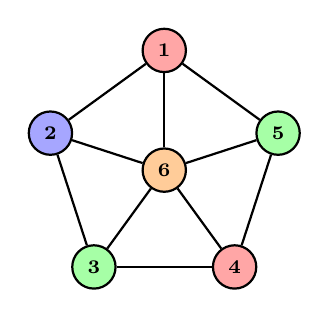
\begin{tikzpicture}[
  vtx/.style={circle,draw,thick,minimum size=0.55cm,font=\scriptsize\bfseries,inner sep=0pt},
  edge/.style={thick},
  scale=0.95,
]
  \node[vtx,fill=red!35]    (v1) at (90:1.6)  {1};
  \node[vtx,fill=blue!35]   (v2) at (162:1.6) {2};
  \node[vtx,fill=green!35]  (v3) at (234:1.6) {3};
  \node[vtx,fill=red!35]    (v4) at (306:1.6) {4};
  \node[vtx,fill=green!35]  (v5) at (18:1.6)  {5};
  \node[vtx,fill=orange!40] (v6) at (0,0) {6};
  \draw[edge] (v1) -- (v2);
  \draw[edge] (v2) -- (v3);
  \draw[edge] (v3) -- (v4);
  \draw[edge] (v4) -- (v5);
  \draw[edge] (v5) -- (v1);
  \draw[edge] (v6) -- (v1);
  \draw[edge] (v6) -- (v2);
  \draw[edge] (v6) -- (v3);
  \draw[edge] (v6) -- (v4);
  \draw[edge] (v6) -- (v5);
\end{tikzpicture}
\end{document}
